\documentclass[12pt,a4paper]{article} %Tipo de documento

%Algunos paquetes nesesarios, deben de ir en preambulo las paqueterias.
\usepackage[spanish]{babel} 
\usepackage[utf8]{inputenc}
\usepackage[numbers,sort&compress]{natbib} %Para la bibliografía
\usepackage{graphicx} %Para incluir figuras
\usepackage{amsfonts}
\usepackage[left=2cm,right=2cm,top=2cm,bottom=2cm]{geometry}
\usepackage{listings}
\usepackage[usenames,dvipsnames]{color}

\lstset{ 
  language=R,
  basicstyle=\scriptsize\ttfamily,
  numbers=left,
  numberstyle=\tiny\color{Blue},
  stepnumber=1,
  numbersep=5pt,
  backgroundcolor=\color{white},
  showstringspaces=false,
  showtabs=false,
  frame=single,
  rulecolor=\color{black},
  tabsize=2,
  captionpos=b,
  breaklines=true,
  breakatwhitespace=false,        
  keywordstyle=\color{RoyalBlue},
  commentstyle=\color{YellowGreen},
  stringstyle=\color{ForestGreen}
}

\title{Matemáticas Computacionales \\ Práctica 1: Gráficas de curvas en R} %Título del documento
\author{1904381 Itzel Guadalupe Vega Yañez \\ Semestre Febrero - Junio 2021} %Autor del documento
\date{16 de Febrero del 2021}

%Hasta aquí es el preambulo, sigue el documento
\begin{document}

\maketitle %Para crear el título del documento

\section{Introducci\'{o}n}\label{sec:intro} %Sección del documento referenciado con 'intro'

En esta primera práctica se hará una de las cosas básicas al momento de aprende R. Se repasaran las curvas en $\mathbb{R}^2$ vistas en primer semestre en la materia de Geometría Analítica\citep{geometria}. Se graficarán curvas como la recta, parábola, circunferencia, elipse e hipérbola.

\section{Curvas de $\mathbb{R}^2$} \label{sec:curvas}

\subsection{Línea recta} \label{subsec:linearecta}

\textbf{Definici\'{o}n}: Llamamos linea recta a1 lugar geometrico de 1os puntos tales que tornados dos puntos diferentes cualesquiera $P_{1}(x_{1},y_{1})$ y $P_{2}(x_{2},y_{2})$ del lugar, el valor de la pendiente $m$ calculado por medio de la formula del teorema 4, Articulo 8,

\begin{equation}
m=y_{1}-y_{2}/x_{1}-x_{2}; x_{1} \neq x_{2},
\end{equation}

resulta siempre constante.
\begin{figure}
\centering
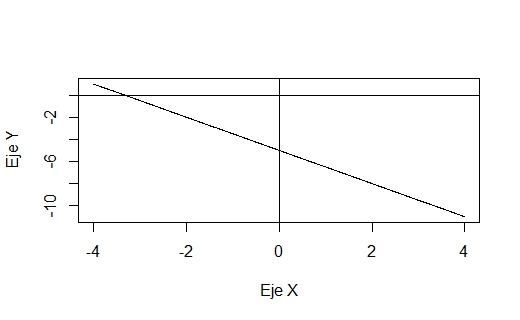
\includegraphics[scale=0.75]{Recta2.png}
\caption{Grafica de linea recta diseño 1; con pendiente -3/2 y pasa por la intersección -5}
\end{figure}

\begin{figure}
\centering
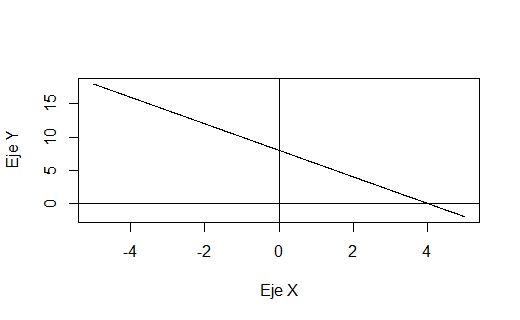
\includegraphics[scale=0.75]{Recta3.png}
\caption{Grafica de linea recta diseño 2; con pendiente -2 y pasa por la intersección 8}
\end{figure}

\subsection{Parábola} \label{subsec:parabola}

\textbf{Definici\'{o}n}: Una parábola es el lugar geométrico de un punto que se mueve en un plano de tal manera que su distancia de una recta fija, situada en el plano, es siempre igual a su distancia de un punto fijo del plano y que no pertenece a la recta. El punto fijo se llama \textit{foco} y la recta fija \textit{directiz} de la parábola.

\begin{figure}
\centering
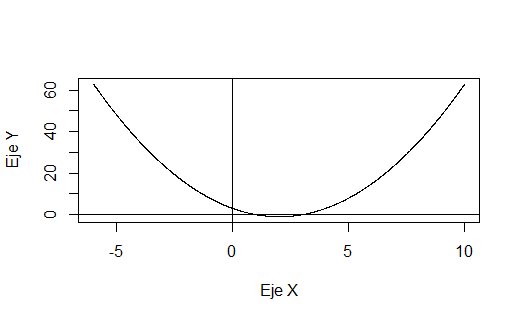
\includegraphics[scale=0.75]{Parabola2.png}
\caption{Grafica de la parabola $y=x^2-4x+3$, diseño 1}
\end{figure}

\begin{figure}
\centering
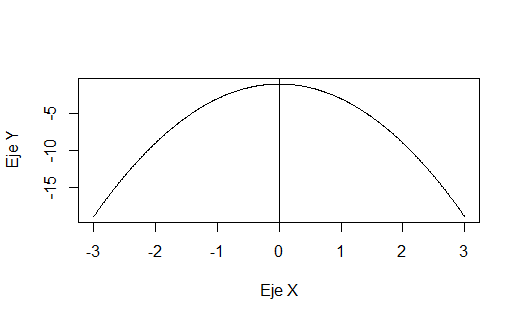
\includegraphics[scale=0.75]{Parabola3.png}
\caption{Grafica de la parabola $y=-2x^2-1$, diseño 2}
\end{figure}

\newpage
\subsection{Circunferencia} \label{subsec:circunferencia}

\textbf{Definici\'{o}n}: Circunferencia es el lugar geométrico de un punto que se mueve en un plano de tal manera que se conserva siempre a unn distancia constante de un punto fijo de ese plano. El punto fijo se llama \textit{centro} de la circunferencia, y la distancia constante se llama \textit{radio}.

\begin{figure}
\centering
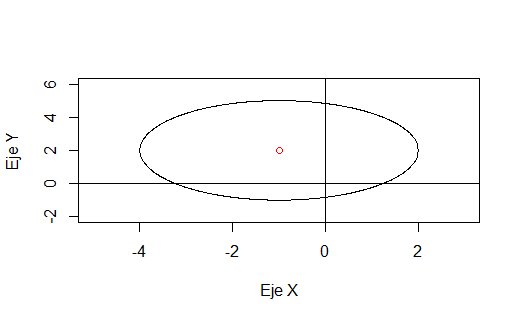
\includegraphics[scale=0.75]{Circunfe2.png}
\caption{Grafica de la circunferencia con centro en (-1,2) y radio 3, diseño 1}
\end{figure}

\begin{figure}
\centering
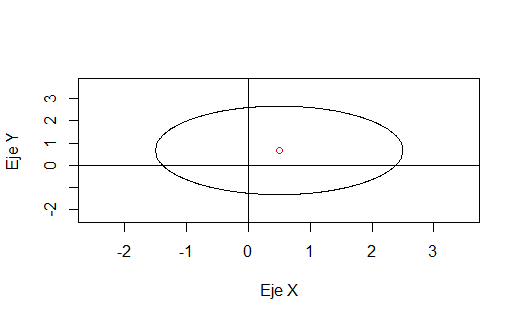
\includegraphics[scale=0.75]{Circunfe3.png}
\caption{Grafica de la circunferencia con centro en (1/2,2/3) y radio 2, diseño 2}
\end{figure}

\subsection{Elipse}

\textbf{Definici\'{o}n}: Una elipse es el lugar geométrico de un punto que se mueve en un plano de tal manera que la suma de sus distancias a dos puntos fijos de ese plano es siempre igual a una constante, mayor que la distancia entre los dos puntos. Los dos puntos fijos se llaman \textit{focos} de la elipse. 

\begin{figure}
\centering
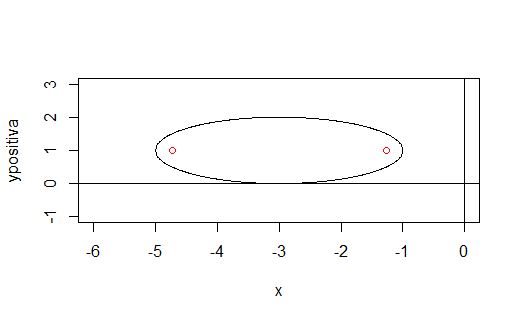
\includegraphics[scale=0.75]{Elipse2.png}
\caption{Grafica de la elipse horizontal con centro en (-3,1), $a = 2$ y $b = 1$, diseño 1}
\end{figure}

\begin{figure}
\centering
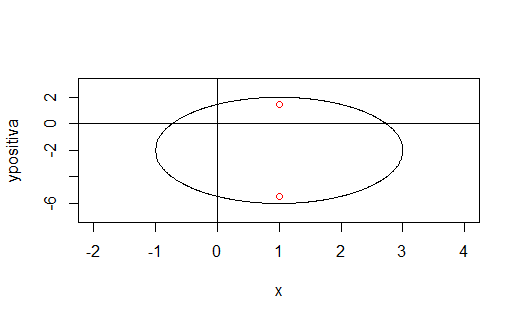
\includegraphics[scale=0.75]{Elipse3.png}
\caption{Grafica de la elipse vertical con centro en (1,-2), $a = 4$ y $b = 2$, diseño 2}
\end{figure}


\newpage
\subsection{Hipérbola}

\textbf{Definici\'{o}n}: Una hipérbola es el lugar geométrico de un punto que se mueve en un plano de tal manera que el valor absoluto de la diferencia de sus distancias a dos puntos fijos del plano, llamados \textit{focos}, es siempre igual a una cantidad constante, positiva y menor que la distancia entre los focos; excluye el caso en que el punto movil se mueva sobre la recta que pasa por los focos a excepción del segmento comprendido entre ellos. Los focos y el punto medio de este segmento no pueden pertenecer al lugar geométrico.

\begin{figure}
\centering
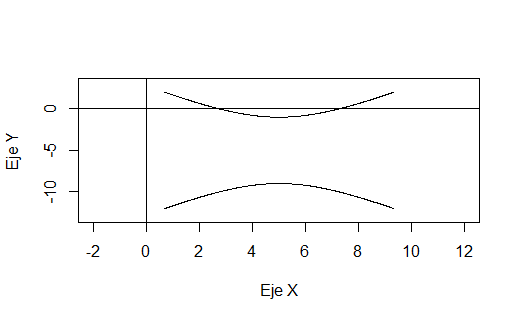
\includegraphics[scale=0.75]{Hiperbola2.png}
\caption{Grafica de la hiperbola sobre el eje Y con centro en (5,-5), $a = 4$ y $b = 3$, diseño 1}
\end{figure}

\begin{figure}
\centering
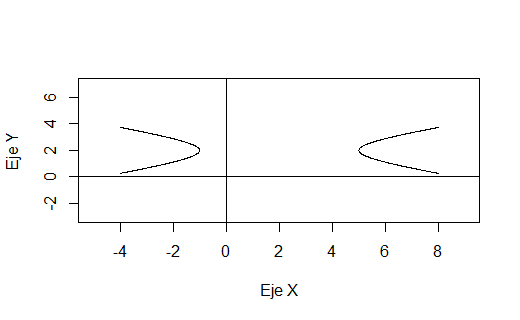
\includegraphics[scale=0.75]{Hiperbola3.png}
\caption{Grafica de la hiperbola sobre el eje Y con centro en (2,2), $a = 3$ y $b = 1$, diseño 2}
\end{figure}

%Bibliografia, recuerda siempre que agregues un referencia nueva compilar el archivo BibTex (con F11 en Texmaker), luego el compilar el .tex
\bibliography{biblio}
\bibliographystyle{plainnat}

\end{document}
